\documentclass[UTF8]{ctexart}
\usepackage{amsmath}
\usepackage{graphicx}
\usepackage{float}
\usepackage{subfigure}
\usepackage{xeCJK}
\usepackage{hyperref}
\usepackage{algorithm2e}
\usepackage{amsfonts}
\usepackage{epsfig}
\usepackage{listings}
\usepackage{xcolor}
% 定义可能使用到的颜色

\definecolor{CPPLight}  {HTML} {686868}
\definecolor{CPPSteel}  {HTML} {888888}
\definecolor{CPPDark}   {HTML} {262626}
\definecolor{CPPBlue}   {HTML} {4172A3}
\definecolor{CPPGreen}  {HTML} {487818}
\definecolor{CPPBrown}  {HTML} {A07040}
\definecolor{CPPRed}    {HTML} {AD4D3A}
\definecolor{CPPViolet} {HTML} {7040A0}
\definecolor{CPPGray}  {HTML} {B8B8B8}
\lstset{
    columns=fixed,
    numbers=left,                                        % 在左侧显示行号
    frame=none,                                          % 不显示背景边框
    backgroundcolor=\color[RGB]{245,245,244},            % 设定背景颜色
    keywordstyle=\color[RGB]{40,40,255},                 % 设定关键字颜色
    numberstyle=\footnotesize\color{darkgray},           % 设定行号格式
    commentstyle=\it\color[RGB]{0,96,96},                % 设置代码注释的格式
    stringstyle=\rmfamily\slshape\color[RGB]{128,0,0},   % 设置字符串格式
    showstringspaces=false,                              % 不显示字符串中的空格
    language=c++,                                        % 设置语言
    morekeywords={alignas,continute,friend,register,true,alignof,decltype,goto,
    reinterpret_cast,try,asm,defult,if,return,typedef,auto,delete,inline,short,
    typeid,bool,do,int,signed,typename,break,double,long,sizeof,union,case,
    dynamic_cast,mutable,static,unsigned,catch,else,namespace,static_assert,using,
    char,enum,new,static_cast,virtual,char16_t,char32_t,explict,noexcept,struct,
    void,export,nullptr,switch,volatile,class,extern,operator,template,wchar_t,
    const,false,private,this,while,constexpr,float,protected,thread_local,
    const_cast,for,public,throw,std},
}

\graphicspath{{images/}}
\setCJKmonofont{Microsoft YaHei}

\title{\Huge{计算机算法设计与分析\\ 线性网络与最大流}}
\author{\Huge{易凯}}
\date{\Huge{2017年6月3日}}

\begin{document}
    \maketitle
    \vspace{35mm}
    \begin{flushright}
    \Large{
    \textbf{班\ \ \ \ \ 级} \makebox[5em][l]{软件53班}

    \textbf{学\ \ \ \ \ 号} \makebox[5em][l]{2151601053}

    \textbf{邮\ \ \ \ \ 箱} \makebox[5em][l]{williamyi96@gmail.com}

    \textbf{联系电话} \makebox[5em][l]{13772103675}

    \textbf{个人网站} \makebox[5em][l]{https://williamyi96.github.io}

                      \makebox[5em][l]{williamyi.tech}

      \textbf{实验日期} \makebox[5em][l]{2017年6月3日}

    \textbf{提交日期} \makebox[5em][l]{2017年6月6日}
    }
    \end{flushright}

    \newpage
  	\tableofcontents
  	\newpage
  	\listoffigures
    \newpage

    \section{线性规划基本定理}
    \subsection{线性规划基本定理}
    如果线性规划问题有最优解,则必有一基本可行解。

    单纯型法是解决线性规划问题的一种有效方法。

    \subsection{单纯型法基本思路}
    先找出一个基本可行解,判断其是否是最优解,如果为否,则切换到相邻的基本可行解,并使目标函数值不断增大,一直找到最优解为止。

    \subsection{单纯型法的特点}
    1. 只对约束条件的若干组合进行测试,测试的每一步都使目标函数的值增加;

    2. 一般经过不大于m或者n次迭代就可求得最优解。

    \section{最大网络流问题}
    \subsection{网络流}
    网络上的流是定义在网络的边集合E上的一个非负函数flow={flow(v,w)},并称flow(v,w)为边(v,w)上的流量

    \subsection{可行流}
    满足下述条件的流flow称为可行流:

    \paragraph{容量约束}   对每一条边(v,w)∈E,0≤flow(v,w)≤cap(v,w)

    \paragraph{平衡约束}   对于中间顶点:流出量=流入量

    \paragraph{边流}    对于网络G的一个给定的可行流flow,将网络中满足flow(v,w)=cap(v,w)的边称为饱和边;flow(v,w)<cap(v,w)的边称为非饱和边;flow(v,w)=0的边称为零流边;flow(v,w)>0的边称为非零流边。当边(v,w)既不是一条零流边也不是一条饱和边时,称为弱流边。

    \paragraph{最大流}
    最大流问题即求网络G的一个可行流flow,使其流量f达到最大。即flow满足:0≤flow(v,w)≤cap(v,w),(v,w)∈E;且

    \begin{figure}[!htb]
      \centering
      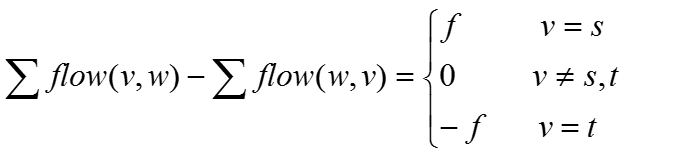
\includegraphics[width=0.8\textwidth]{../img/8.1.png}
      \caption{最大流}\label{最大流}
    \end{figure}

    \paragraph{流的费用}
    在实际应用中,与网络流有关的问题,不仅涉及流量,而且还有费用的因素。此时网络的每一条边(v,w)除了给定容量cap(v,w)外,还定义了一个单位流量费用cost(v,w)。对于网络中一个给定的流flow,其费用定义为:

    \begin{figure}[!htb]
      \centering
      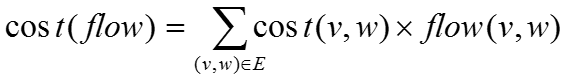
\includegraphics[width=0.8\textwidth]{../img/8.2.png}
      \caption{流的费用}\label{流的费用}
    \end{figure}

    相关的更多算法以及定义的概念详情参照书本内容。在此不进行赘述。
\end{document} 